\documentclass[11pt]{article}
\usepackage[margin=1in]{geometry}
\usepackage{graphicx}
\usepackage{subcaption}
\usepackage{booktabs}
\usepackage{amsmath}
\usepackage{amssymb}
\usepackage{siunitx}
% after \usepackage{siunitx}
\DeclareSIUnit\px{px}
\usepackage{enumitem}
\usepackage{xcolor}
\usepackage{float} 
\usepackage{placeins}
\usepackage[utf8]{inputenc}
\usepackage{hyperref}
\hypersetup{colorlinks=true,linkcolor=blue,citecolor=blue,urlcolor=blue}


% ==== Project macros (fill in your name/date if different) ====
\title{Mini-Project 1: Image Classification on Caltech-101}
\author{Luc Chen}
\date{October 2025}

% Results macros (update here if you rerun models)

\newcommand{\accEffb}{0.924}\newcommand{\macroEffb}{0.916}\newcommand{\wFOneEffb}{0.922}\newcommand{\topFiveEffb}{0.995}
\newcommand{\accRes}{0.901}\newcommand{\macroRes}{0.889}\newcommand{\wFOneRes}{0.900}\newcommand{\topFiveRes}{0.991}
\newcommand{\accViT}{0.848}\newcommand{\macroViT}{0.822}\newcommand{\wFOneViT}{0.835}\newcommand{\topFiveViT}{0.975}
\newcommand{\accHOG}{0.137}\newcommand{\macroHOG}{0.017}\newcommand{\wFOneHOG}{0.081}
\newcommand{\accRF}{0.465}\newcommand{\macroRF}{0.229}\newcommand{\wFOneRF}{0.394}

% === Helper macros for tidy appendix plots ===
% A compact 2x2 panel: train acc, val acc, val macro-F1, confusion matrix
\newcommand{\ResultPanel}[3]{%
  % #1 = run folder under results/ (e.g., resnet18_224_sgd_cosine_ls01)
  % #2 = short model name for caption (e.g., ResNet-18 (224px, cosine+LS0.1))
  % #3 = optional extra caption text (can be empty)
  \begin{figure}[H]
    \centering
    \begin{subfigure}[t]{0.49\textwidth}
      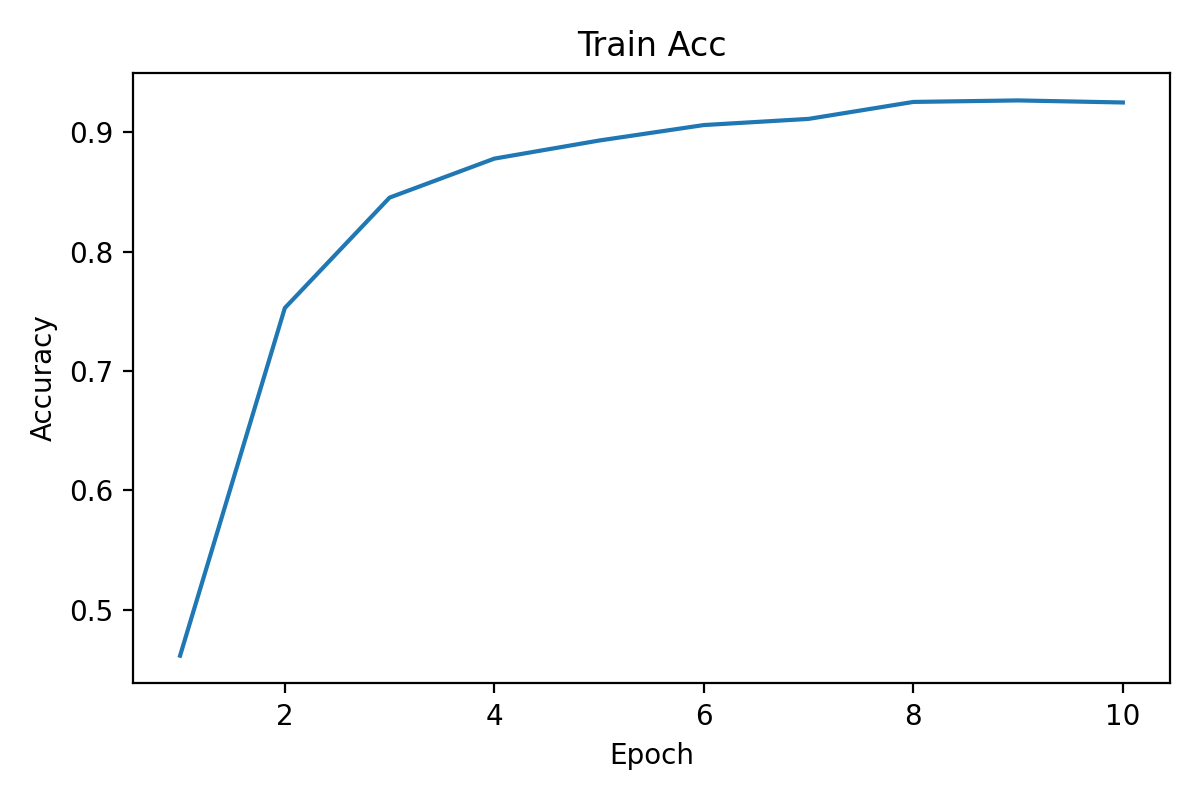
\includegraphics[width=\linewidth]{results/#1/train_acc.png}
      \caption{Train accuracy}
    \end{subfigure}\hfill
    \begin{subfigure}[t]{0.49\textwidth}
      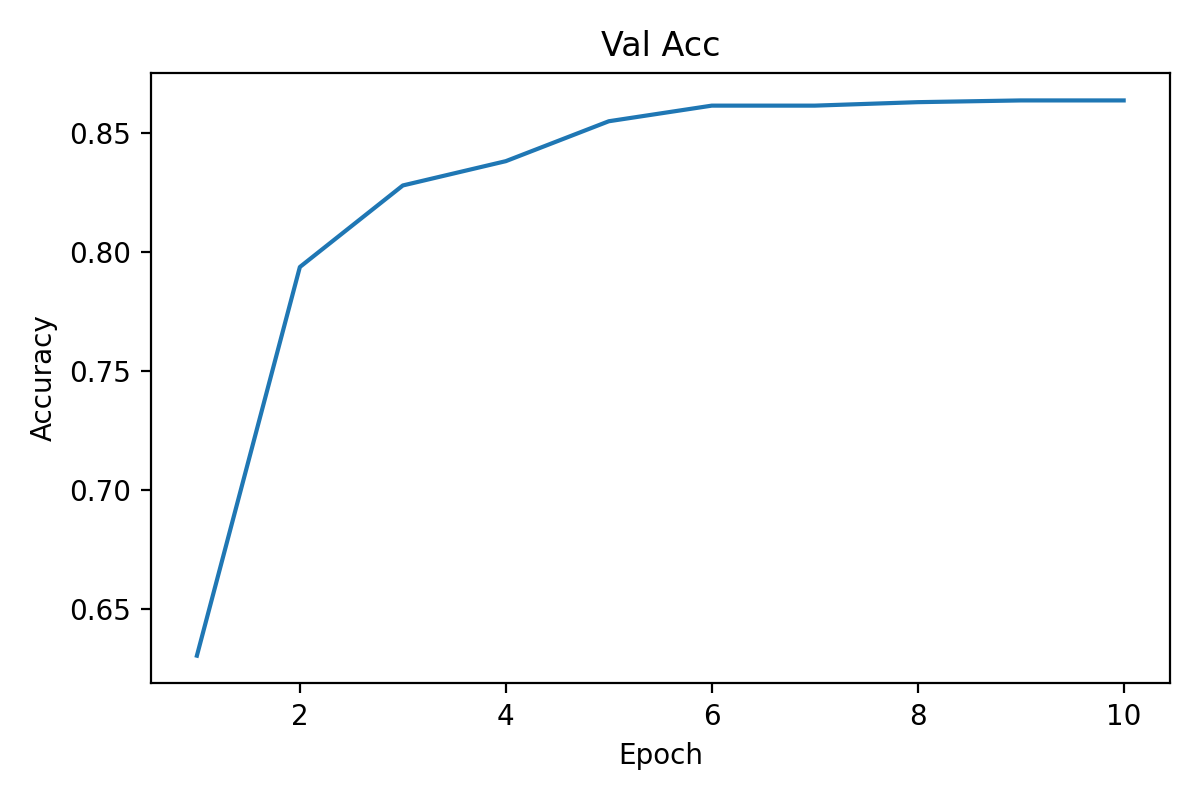
\includegraphics[width=\linewidth]{results/#1/val_acc.png}
      \caption{Validation accuracy}
    \end{subfigure}

    \vspace{0.35em}

    \begin{subfigure}[t]{0.49\textwidth}
      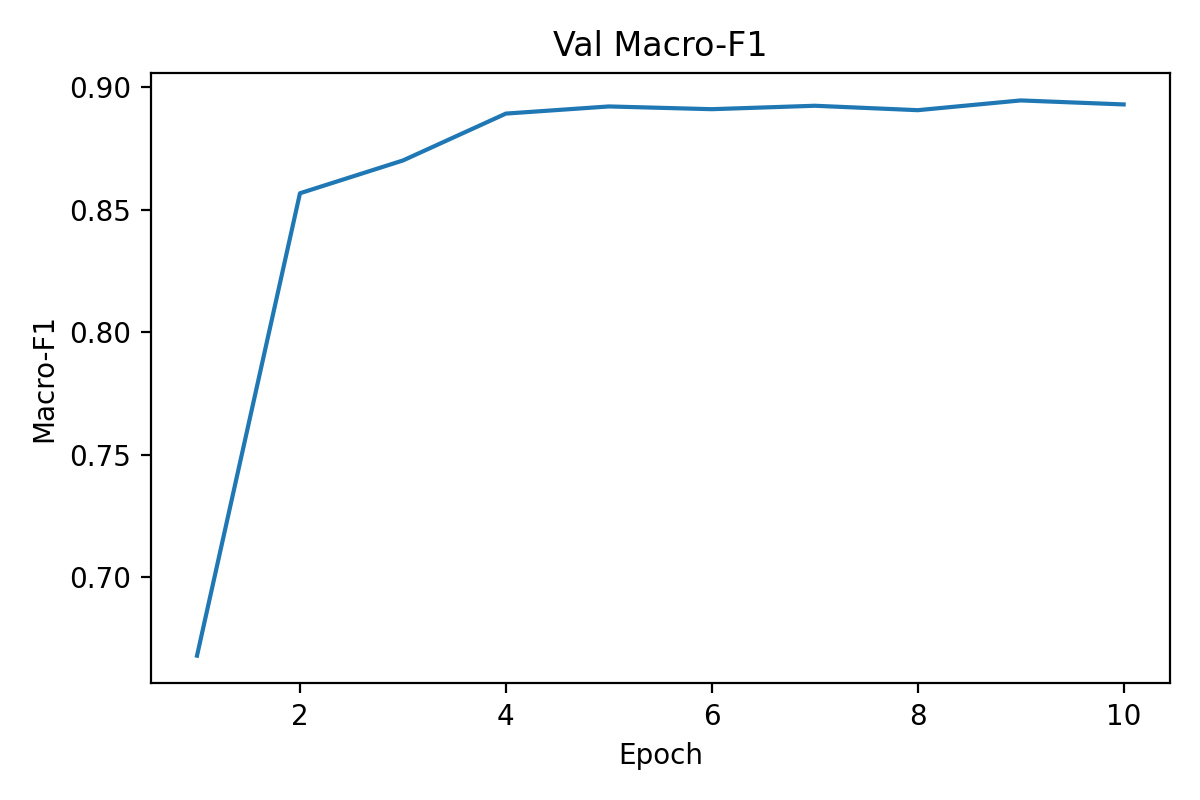
\includegraphics[width=\linewidth]{results/#1/val_macro_f1.png}
      \caption{Validation macro-F1}
    \end{subfigure}\hfill
    \begin{subfigure}[t]{0.49\textwidth}
      \includegraphics[width=\linewidth]{results/#1/confusion_matrix.png}
      \caption{Confusion matrix}
    \end{subfigure}

    \caption{#2. #3}
    \label{fig:#1-panel}
  \end{figure}
  \FloatBarrier
}

% A single, centered confusion matrix (for classical baselines to avoid clutter)
\newcommand{\ConfOnly}[2]{%
  % #1 = run folder under results/ (e.g., hog_svm_rbf)
  % #2 = short model name for caption
  \begin{figure}[H]
    \centering
    \includegraphics[width=0.66\textwidth]{results/#1/confusion_matrix.png}
    \caption{Confusion matrix for #2.}
    \label{fig:#1-cm}
  \end{figure}
  \FloatBarrier
}

\begin{document}
\maketitle



\begin{abstract}
\noindent
This report compares classical and modern approaches to object recognition on the Caltech-101 dataset ($\sim$9k images, 101 object categories, plus the common ``BACKGROUND\_Google'' class). We benchmark a traditional HOG+SVM pipeline against three pretrained deep architectures: ResNet-18, EfficientNet-B0, and ViT-B/16, each fine-tuned on stratified 70/15/15 splits. Evaluation metrics include overall accuracy, macro/weighted F1, Top-5 accuracy, and per-class confusion analyses. EfficientNet-B0 achieves the best performance with 0.924 accuracy and 0.916 macro-F1, outperforming classical baselines by a wide margin. Ablation studies on input resolution, data augmentation, and transformer fine-tuning demonstrate how architectural design and training strategy affect generalization under limited data. Overall, the results highlight the continuing advantage of pretrained CNNs and transformers over handcrafted features, while emphasizing practical considerations for small-scale transfer learning.
\end{abstract}

\vspace{1em}


\section{Introduction}
The Caltech-101 benchmark \cite{FeiFei2004} has long served as a compact yet challenging testbed for visual recognition under class imbalance and limited training data. Before deep learning, pipelines built on handcrafted descriptors, such as Histograms of Oriented Gradients (HOG) \cite{Dalal2005} combined with Support Vector Machines (SVMs) \cite{Cortes1995}, formed the foundation of object recognition research. The advent of convolutional neural networks (CNNs) such as ResNet \cite{He2016}, along with more parameter-efficient architectures like EfficientNet \cite{Tan2019} and the emergence of Vision Transformers (ViT) \cite{Dosovitskiy2021}, fundamentally shifted the field toward learned hierarchical representations.

In this project, we revisit Caltech-101 through a unified experimental framework that contrasts classical handcrafted features and ensemble methods with modern pretrained deep models. Specifically, we (i) create stratified 70/15/15 train/validation/test splits, including the common \texttt{BACKGROUND\_Google} class for reproducibility, (ii) evaluate classical baselines (HOG+SVM and HOG+color with Random Forest) alongside three pretrained models: ResNet-18, EfficientNet-B0, and ViT-B/16, (iii) analyze results using accuracy, macro/weighted F1, Top-5 accuracy, per-class accuracy, and confusion structure, and (iv) perform ablation studies on image resolution, data augmentation, and transformer fine-tuning strategies. All experiments are selected by validation macro-F1 to mitigate class imbalance, and full code, figures, and outputs are available in an open repository.

Our results quantify the continuing performance gap between handcrafted and learned representations on Caltech-101, clarify when ViTs require full-layer adaptation to compete with CNNs, and offer practical insights on efficient transfer learning setups for small- to medium-scale datasets.

\section{Dataset and Splits}
The Caltech-101 dataset \cite{FeiFei2004} comprises images from 101 object categories, with significant variation in class frequency and intra-class appearance. Following the project guidelines, we construct stratified splits with 70\% of images for training, 15\% for validation, and 15\% for testing. Stratification ensures balanced representation of all classes across splits and provides a stable validation set for checkpoint selection.

The version of the dataset used in this work includes the additional \texttt{BACKGROUND\_Google} category commonly distributed in public releases.\footnote{Dataset available at \url{https://data.caltech.edu/records/mzrjq-6wc02}} We retain this category as an independent class, resulting in 102 total categories and consistent with most contemporary evaluations \cite{Dalal2005,FeiFei2004}. 

All images are resized to a uniform input size per experiment. For deep models, we apply ImageNet normalization and lightweight data augmentation (random resized crop, horizontal flip, mild color jitter). Training selection is based on validation macro-F1 to address class imbalance and to maintain consistency across model families.
\section{Methods}
\subsection{Classical: HOG + SVM}
As a classical baseline, we implemented the widely used Histogram of Oriented Gradients (HOG) descriptor \cite{Dalal2005} combined with a Support Vector Machine (SVM) classifier \cite{Cortes1995}. 
We extract grayscale HOG features (9 orientations, $8 \times 8$ pixels per cell, $2 \times 2$ cells per block) from images resized to \SI{128}{px}. 
Hyperparameters ($C$ and, for RBF kernels, $\gamma$) are tuned with 3-fold cross-validation on the training+validation set. 

This pipeline historically provided strong performance on tasks such as pedestrian detection and rigid object recognition, and it is computationally efficient compared to modern deep models. 
However, HOG features are handcrafted and primarily capture local edge statistics, making them sensitive to pose, scale, and background variation. 
We include this method not with the expectation of competitive accuracy on Caltech-101, but to serve as a reference point: a core goal of this project is to demonstrate how state-of-the-art deep networks dramatically outperform traditional feature-based pipelines under the same experimental protocol. 

\subsection{Classical+: HOG(+Color) + Random Forest}
To push a traditional pipeline further, we combined handcrafted features with an ensemble classifier.
We extracted grayscale HOG descriptors (same settings as above) and concatenated a simple color
summary: three \emph{HSV} histograms (32 bins/channel), L1-normalized and appended to the HOG vector.
We then trained a Random Forest classifier \cite{Breiman2001} with a small grid over
$n_{\text{estimators}}\in\{300,600,900\}$, $\text{max\_depth}\in\{20,30\}$, and
$\text{max\_features}\in\{\texttt{sqrt},\texttt{log2}\}$, selecting the best model by validation macro-F1.
This enhanced classical setup improves substantially over HOG+SVM, showing that color and ensemble averaging
can recover some invariances (illumination, background), though it still lags behind pretrained CNNs on
fine-grained categories.


\subsection{Deep: Transfer Learning}
To evaluate modern approaches, we fine-tune pretrained deep architectures with a new classification head. 
Each backbone represents a distinct family of design choices that are widely used in contemporary vision systems:

\begin{itemize}[leftmargin=*]
  \item \textbf{ResNet-18} \cite{He2016}: a residual CNN that introduced skip connections to ease optimization of deep networks. 
  We adopt it as a canonical convolutional baseline, trained with SGD with momentum, cosine learning-rate scheduling \cite{Loshchilov2017}, and label smoothing \cite{Szegedy2016}. 
  
  \item \textbf{EfficientNet-B0} \cite{Tan2019}: a scaled CNN designed with compound depth/width/resolution scaling. 
  It is more parameter-efficient than ResNet for similar accuracy, making it a strong representative of modern CNNs. 
  We train it with Adam \cite{Kingma2015} and cosine scheduling. 
  
  \item \textbf{ViT-B/16} \cite{Dosovitskiy2021}: a Vision Transformer that replaces convolutions with self-attention over $16 \times 16$ image patches. 
  As transformers are known to require larger datasets, we include a frozen-backbone variant (only the head is trained) and compare it to full fine-tuning in ablations. 
  This illustrates trade-offs between compute budget and accuracy.
\end{itemize}

All models are initialized from ImageNet-1k pretrained weights and fine-tuned on Caltech-101 for 10 epochs with batch size 64 unless otherwise noted. 
In addition to standard Top-1 accuracy, we also report Top-5 accuracy to capture whether models consistently rank the correct class among their highest-confidence predictions.

\section{Experimental Setup}

\textbf{Preprocessing.} 
We resized inputs to match the common pretraining resolutions of each backbone: \SI{224}{px} for EfficientNet and ViT, and \SI{128}{px} or \SI{224}{px} for ResNet ablations. 
When we first tried lower resolutions, we noticed faster training but weaker fine-grained recognition (e.g., distinguishing similar instruments or animals). 
We therefore kept \SI{224}{px} as the default for the main experiments. 
All inputs are normalized with ImageNet mean and variance so that pretrained weights remain compatible.

\textbf{Augmentation.} 
We included RandomResizedCrop, HorizontalFlip, and mild ColorJitter. 
In early runs without augmentation, validation accuracy rose quickly but generalization dropped, especially for classes with fewer samples. 
Adding light augmentation made training slightly noisier at first but improved macro-F1 by making the models more robust to pose and background variation.

\textbf{Optimization.} 
We compared Adam \cite{Kingma2015} (lr $3\times 10^{-4}$) and SGD with momentum 0.9 (lr 0.01). 
Initially, Adam converged faster and was easier to tune, especially for EfficientNet. 
However, for ResNet, we observed that SGD with a cosine learning-rate schedule \cite{Loshchilov2017} led to smoother learning curves and better final accuracy. 
We also applied label smoothing (0.05–0.1) \cite{Szegedy2016} after seeing that some models became overconfident, which harmed macro-F1 on minority classes.

\textbf{Model selection.} 
Rather than selecting checkpoints by accuracy, we chose the model with the best validation macro-F1. 
We realized that accuracy was dominated by frequent categories, while macro-F1 gave a fairer view across all 102 classes, especially for those with limited examples. 
Final test metrics are always reported from the best validation-F1 checkpoint, to avoid bias from training noise or overfitting.

\textbf{Ablation variations.} 
In addition to this default pipeline, we also explored controlled variations in image resolution, augmentation strength, and optimization strategy. 
These are presented later in Section~\ref{section:Ablation}.


\section{Results}
\subsection{Overall Metrics}
Table~\ref{tab:overall} summarizes quantitative results on the Caltech-101 test set.
Across all models, pretrained deep networks outperform classical pipelines by a wide margin.
EfficientNet-B0 achieves the highest Top-1 accuracy (\accEffb{}) and macro-F1 (\macroEffb{}),
while ResNet-18 remains competitive with \accRes{} accuracy and \macroRes{} macro-F1.
ViT-B/16, when trained with a frozen backbone for only 10 epochs, slightly underperforms the CNNs
but still greatly exceeds the handcrafted feature baselines.
These findings are consistent with expectations that transformers require either
larger datasets or longer fine-tuning schedules to realize their full potential.

Classical feature-based methods lag far behind: HOG+SVM achieves only \accHOG{} accuracy,
roughly 13$\times$ above random guessing but an order of magnitude below CNNs.
Adding color histograms and switching to a Random Forest classifier
improves to \accRF{} accuracy and \macroRF{} macro-F1, showing that
ensemble averaging and color cues provide modest robustness gains,
though they remain limited in representing complex intra-class variation.

\begin{table}[h]
  \centering
  \begin{tabular}{lcccc}
    \toprule
    Method & Acc & Macro-F1 & W-F1 & Top-5 \\
    \midrule
    HOG+SVM (RBF) & \accHOG & \macroHOG & \wFOneHOG & -- \\
    {RF (HOG+color)} & \accRF & \macroRF & \wFOneRF & -- \\
    ResNet-18 & \accRes & \macroRes & \wFOneRes & \topFiveRes \\
    EfficientNet-B0 & \accEffb & \macroEffb & \wFOneEffb & \topFiveEffb \\
    ViT-B/16 (frozen) & \accViT & \macroViT & \wFOneViT & \topFiveViT \\
    \bottomrule
  \end{tabular}
  \caption{Test metrics on Caltech-101. W-F1 denotes weighted F1.}
  \label{tab:overall}
\end{table}

\subsection{Per-class Accuracy and Confusion}
Per-class accuracy for a class $c$ is
\[
a_c \;=\; \frac{1}{|\mathcal{D}_c|}\sum_{(x,y)\in\mathcal{D}_c} \mathbf{1}\,[\hat{y}=y=c],
\]
which isolates performance on each category regardless of class frequency. In addition to the macro/weighted
F1 scores in Table~\ref{tab:overall}, we use per-class accuracy and the confusion matrix to diagnose
imbalance-driven failures. Figure~\ref{fig:cms} compares confusion matrices across all evaluated models,
and Appendix~\ref{app:perclass} reports the \emph{Top/Bottom-5 per-class accuracies} for each model.

\paragraph{Classical baselines.}
The classical models in Fig.~\ref{fig:cms} (top row) illustrate the limitations of handcrafted features on Caltech-101.
The HOG+SVM baseline shows a faint main diagonal with widespread off-diagonal errors, reflecting strong bias toward
dominant categories such as \emph{BACKGROUND\_Google} and poor generalization to diverse object types.
Adding color histograms and replacing the SVM with a Random Forest yields a visibly denser diagonal and fewer
background confusions, indicating that ensemble averaging and simple color cues help separate broad visual groups
(e.g., animals, flowers, vehicles). Nonetheless, both methods exhibit substantial misclassification among
fine-grained or structurally similar categories, underscoring the limits of handcrafted representations.

\paragraph{Deep transfer models.}
The pretrained CNN and transformer models (Fig.~\ref{fig:cms}, bottom row) produce much sharper diagonals with minimal
off-diagonal scatter, confirming their superior generalization across classes. ResNet-18 and EfficientNet-B0 achieve
strong, uniformly distributed accuracy with few category-level confusions. Their remaining errors typically involve
visually ambiguous or cluttered classes (e.g., \emph{lotus}, \emph{lobster}). ViT-B/16 with a frozen backbone also
exhibits a clean diagonal but lower contrast in rare or fine-grained categories, consistent with under-adaptation of
its attention layers to limited data. In later ablations, full fine-tuning of ViT substantially improves these cases,
demonstrating that transformer-based architectures require greater representational flexibility than CNNs to perform
optimally at this scale.

% === Confusion matrices (ensure these files exist in your Overleaf project) ===
\begin{figure}[H]
  \centering

  % --- Classical ---
  \begin{subfigure}[t]{0.32\textwidth}
    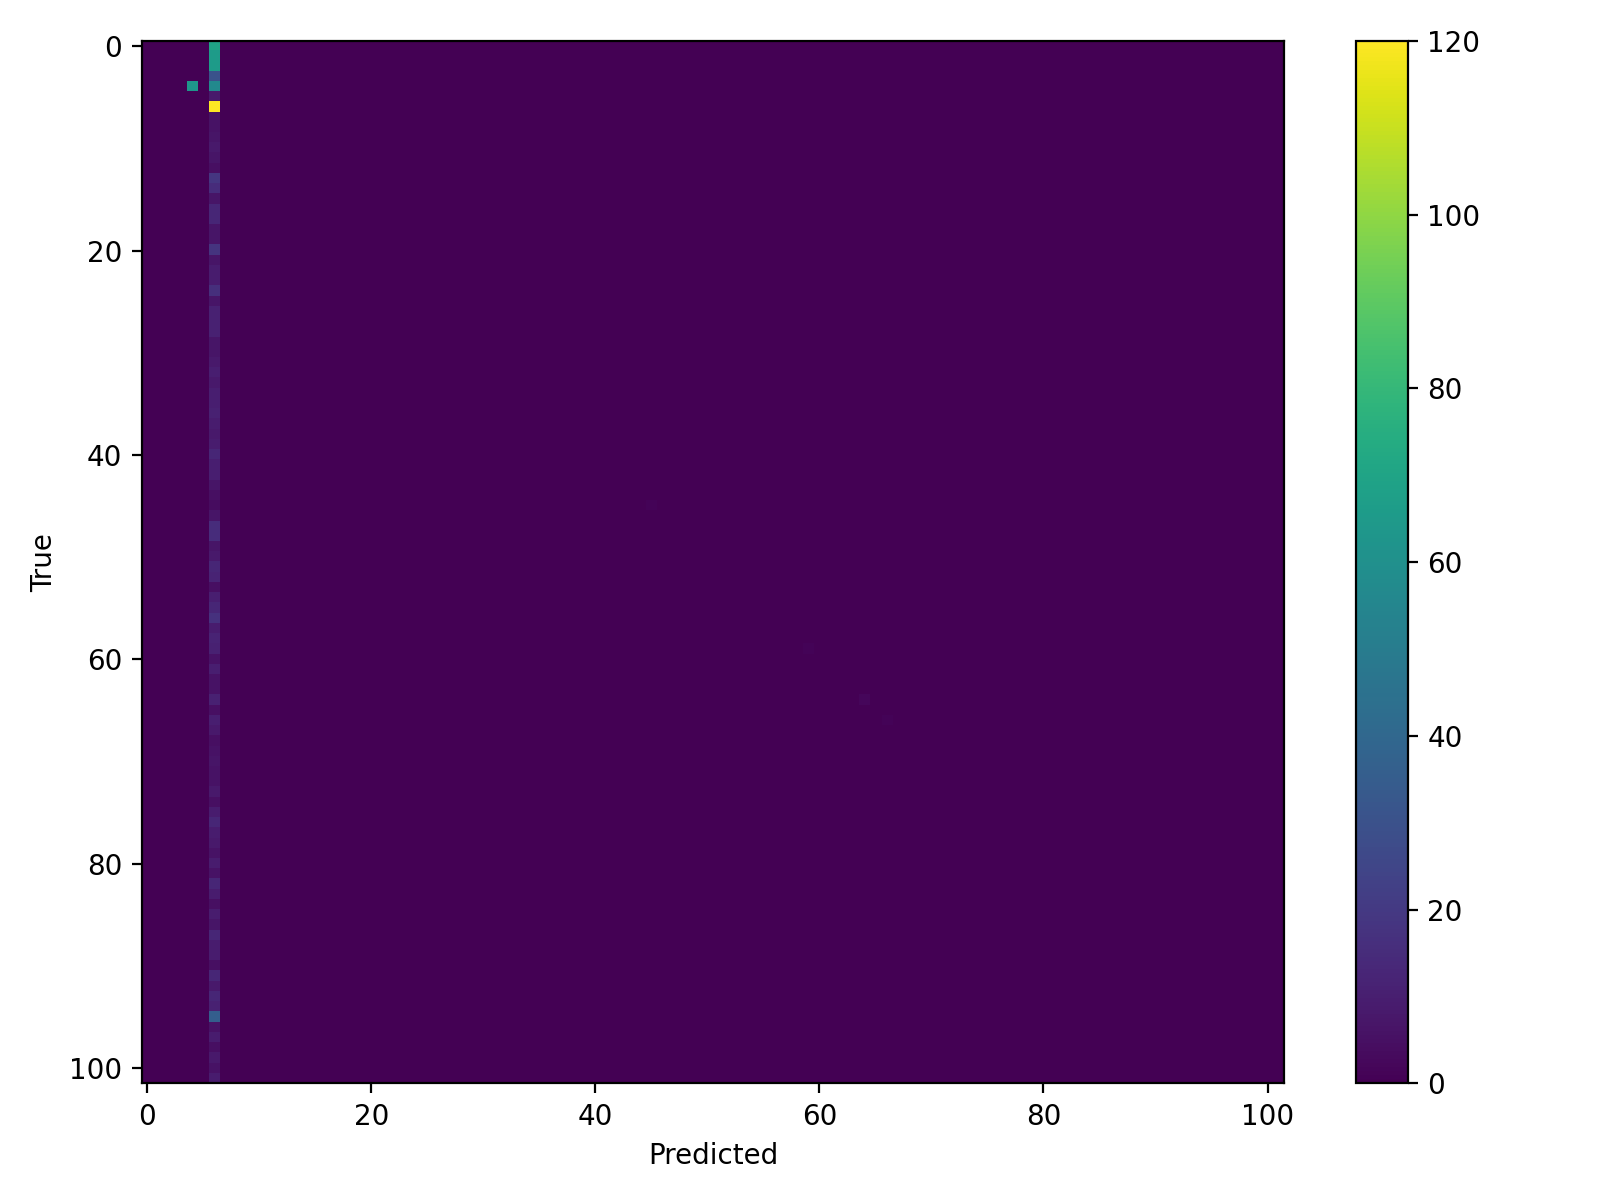
\includegraphics[width=\linewidth]{results/hog_svm_rbf/confusion_matrix.png}
    \caption{HOG+SVM}\label{fig:cms-hog}
  \end{subfigure}\hfill
  \begin{subfigure}[t]{0.32\textwidth}
    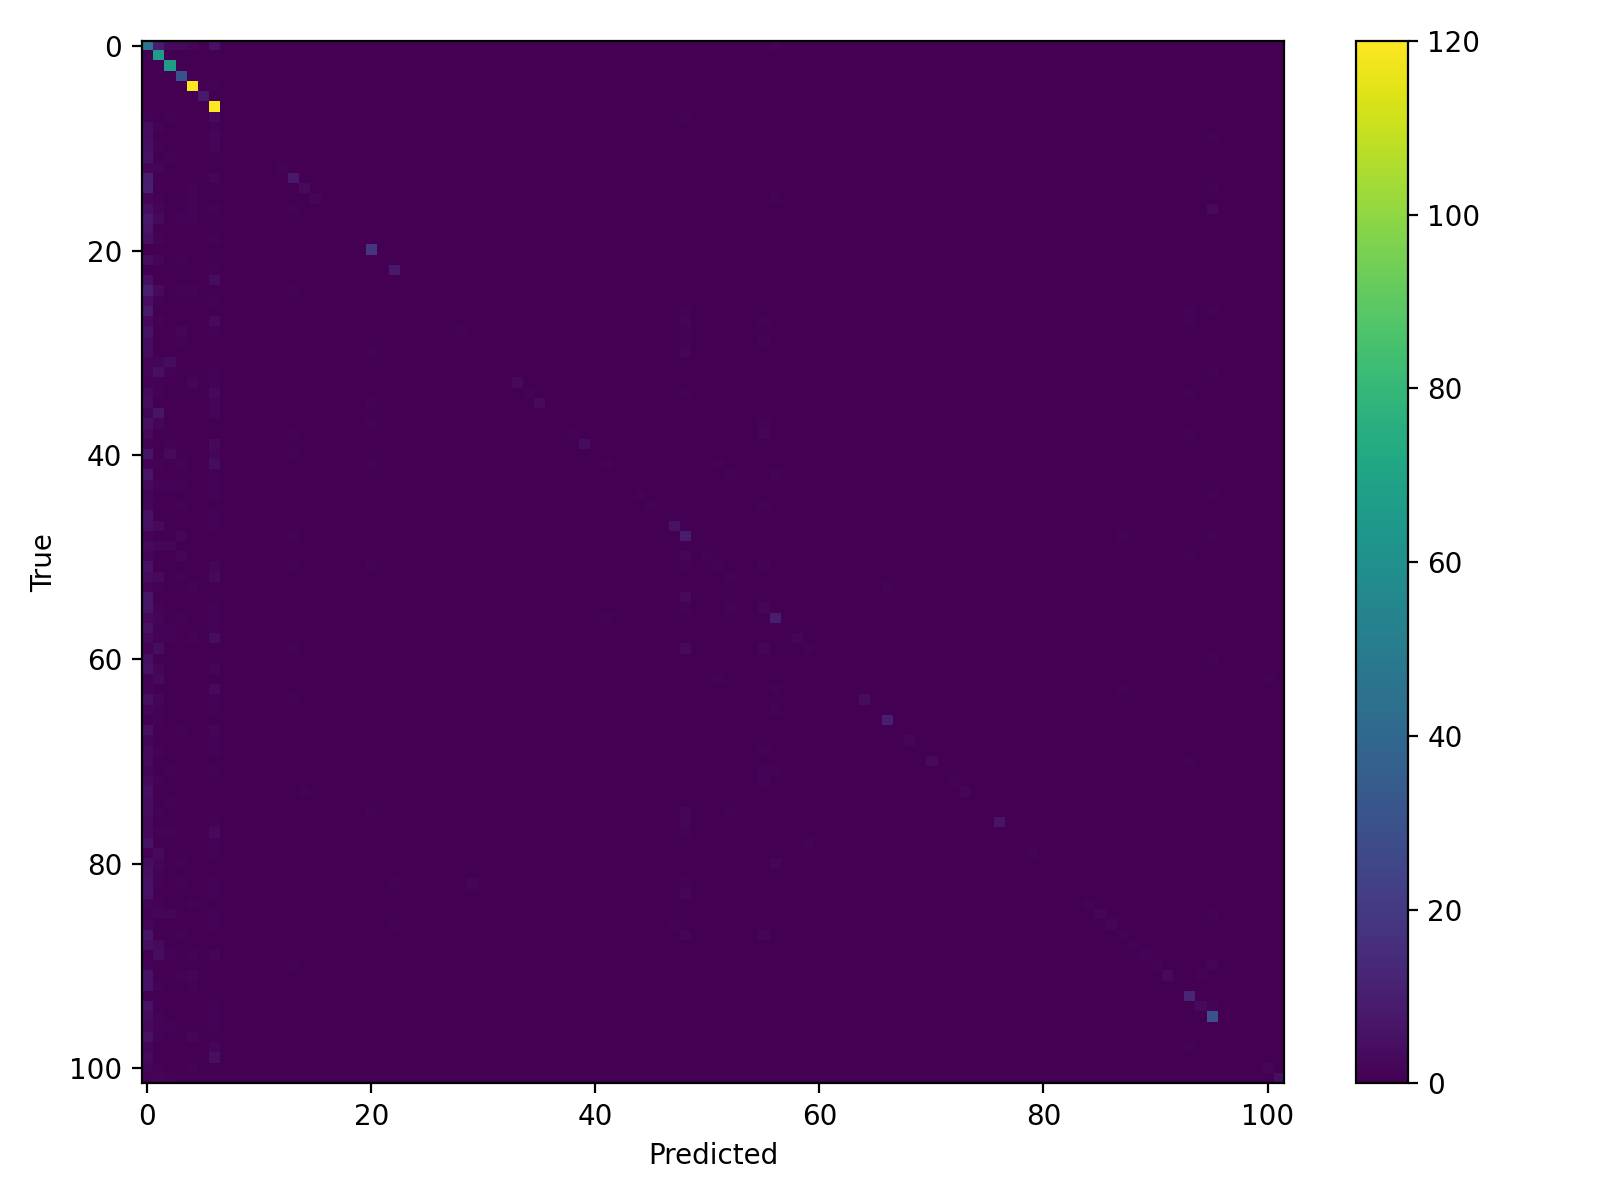
\includegraphics[width=\linewidth]{results/rf_hog_color_128px/confusion_matrix.png}
    \caption{RF (HOG+color)}\label{fig:cms-rf}
  \end{subfigure}

  \vspace{0.5em}

  % --- Deep models ---
  \begin{subfigure}[t]{0.32\textwidth}
    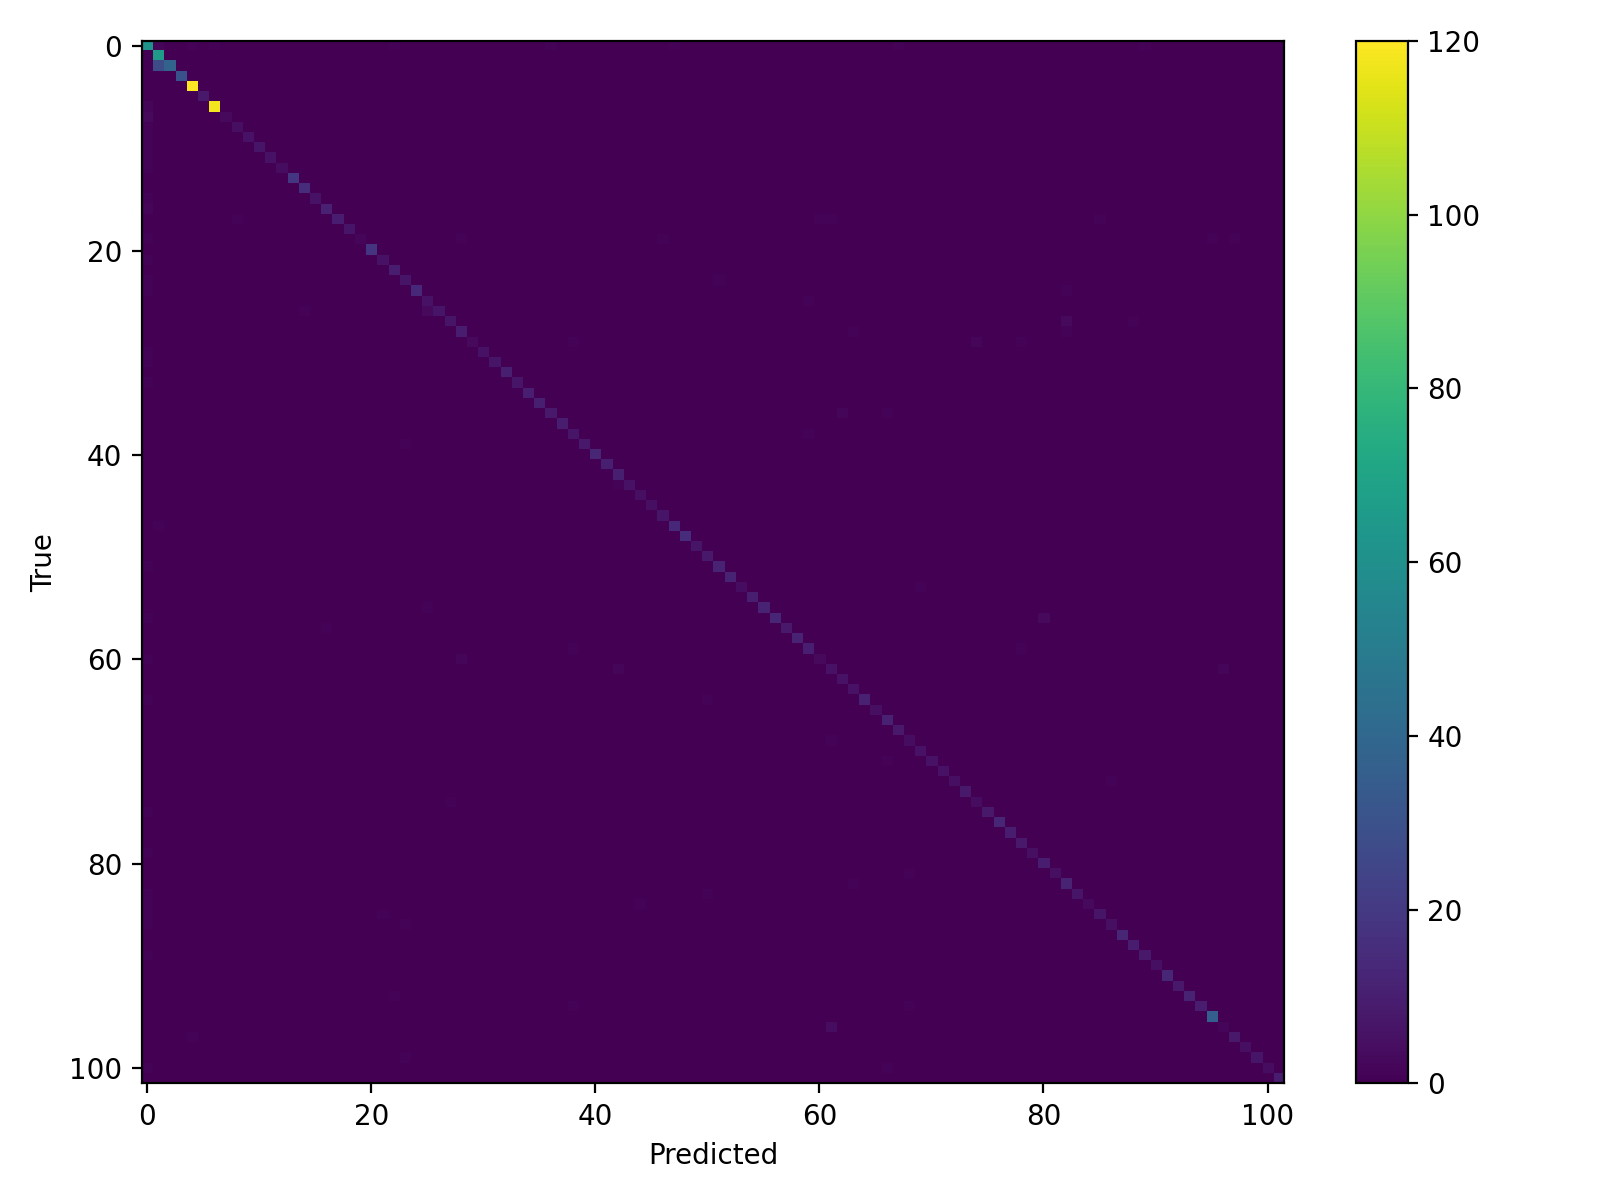
\includegraphics[width=\linewidth]{results/resnet18_224_sgd_cosine_ls01/confusion_matrix.png}
    \caption{ResNet-18}\label{fig:cms-resnet}
  \end{subfigure}\hfill
  \begin{subfigure}[t]{0.32\textwidth}
    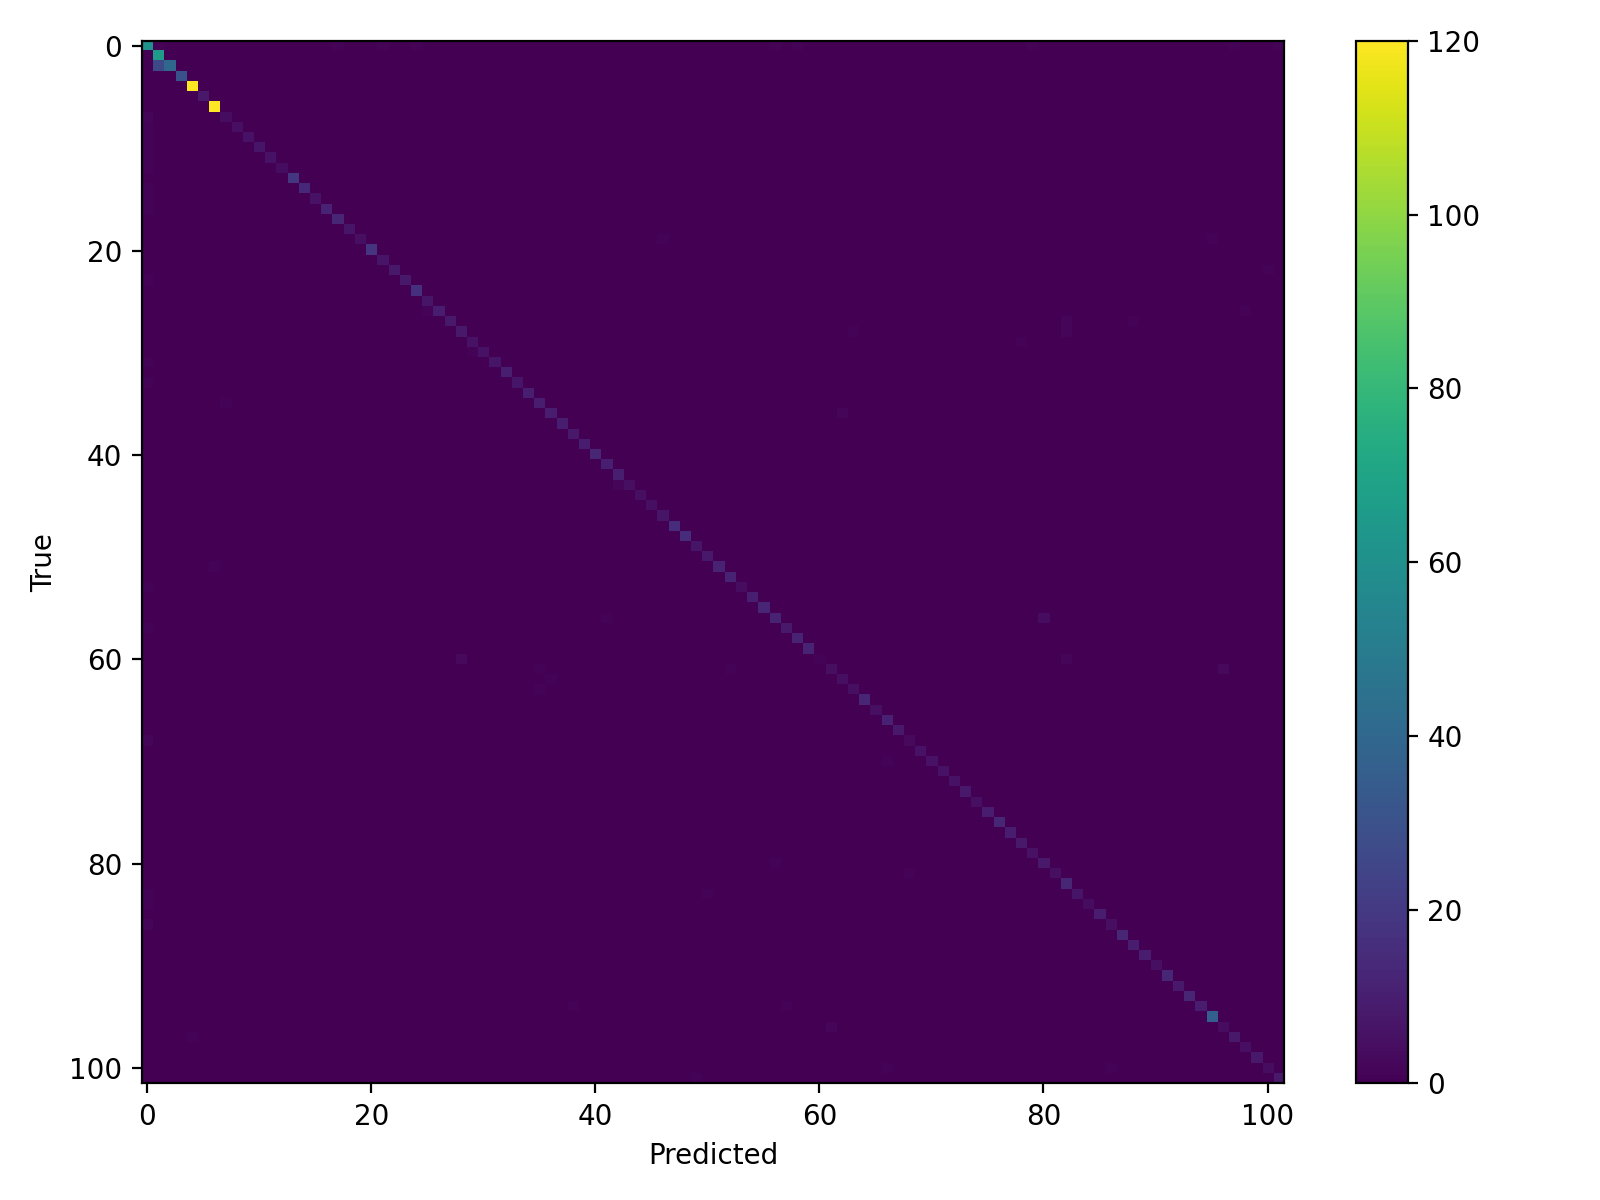
\includegraphics[width=\linewidth]{results/effb0_224_adam_cosine_ls05/confusion_matrix.png}
    \caption{EfficientNet-B0}\label{fig:cms-effb0}
  \end{subfigure}\hfill
  \begin{subfigure}[t]{0.32\textwidth}
    \includegraphics[width=\linewidth]{results/vitb16_224_freeze/confusion_matrix.png}
    \caption{ViT-B/16 (frozen)}\label{fig:cms-vit}
  \end{subfigure}

  \caption{Confusion matrices on the Caltech-101 test set.
  Top: classical methods. Bottom: deep transfer-learning models.
  RF (HOG+color) improves upon HOG+SVM with a clearer diagonal and fewer background confusions,
  though deep pretrained models still achieve the cleanest diagonals and minimal inter-class errors.}
  \label{fig:cms}
\end{figure}



\section{Ablation Studies}
\label{section:Ablation}


We conduct controlled ablations on input resolution, data augmentation, and Vision Transformer fine-tuning strategy.
Each study varies one factor at a time while keeping all other hyperparameters and data splits constant.

\paragraph{A1: Image Size (64 vs.\ 128 vs.\ 224).}
Table~\ref{tab:abl_image_size} shows the effect of input resolution on ResNet-18.
As expected, smaller inputs reduce computational cost but severely degrade fine-grained recognition.
At \SI{64}{px}, accuracy drops to 0.76 with a macro-F1 of only 0.69, confirming that low resolution
obscures discriminative textures and shape cues.
Performance improves sharply at \SI{128}{px} (0.867 accuracy) and saturates near \SI{224}{px} (0.901).
This diminishing return is typical of pretrained CNNs: once the receptive field sufficiently covers object scale,
further resolution increases add redundancy without new signal.
It also indicates that Caltech-101 objects are large enough that most discriminative content
fits comfortably within the 128–224~px range.

\begin{table}[H]
  \centering
  \begin{tabular}{lcccc}
    \toprule
    \textbf{Image Size / Model} & \textbf{Acc} & \textbf{Macro-F1} & \textbf{Weighted-F1} & \textbf{Top-5} \\
    \midrule
    ResNet-18 (64×64)  & 0.760 & 0.688 & 0.757 & 0.932 \\
    ResNet-18 (128×128) & 0.867 & 0.839 & 0.867 & 0.972 \\
    ResNet-18 (224×224) & 0.901 & 0.889 & 0.900 & 0.991 \\
    \bottomrule
  \end{tabular}
  \caption{Effect of input image resolution on ResNet-18 performance.}
  \label{tab:abl_image_size}
\end{table}

\paragraph{A2: Data Augmentation (on vs.\ off).}
We next evaluate how augmentation affects generalization (Table~\ref{tab:abl_augmentation}).
Disabling augmentation yields slightly higher training accuracy but poorer macro-F1 (0.894 vs.\ 0.837),
suggesting overfitting to frequent categories.
Although the absolute accuracy gap (0.921 vs.\ 0.867) is modest, the improvement in macro-F1
demonstrates that augmentation primarily benefits minority classes by introducing intra-class variability.
This aligns with prior work \cite{Szegedy2016}, which found that even mild transformations
can stabilize validation loss and reduce prediction entropy.
A counterintuitive observation is that augmentation’s quantitative gains are small;
this occurs because pretrained ImageNet models already encode many invariances,
so augmentation refines class balance rather than total accuracy.

\begin{table}[H]
  \centering
  \begin{tabular}{lcccc}
    \toprule
    \textbf{Augmentation Setting / Model} & \textbf{Acc} & \textbf{Macro-F1} & \textbf{Weighted-F1} & \textbf{Top-5} \\
    \midrule
    ResNet-18 (no augmentation) & 0.921 & 0.894 & 0.921 & 0.988 \\
    ResNet-18 (with augmentation) & 0.867 & 0.837 & 0.866 & 0.974 \\
    \bottomrule
  \end{tabular}
  \caption{Impact of data augmentation on ResNet-18. Augmentation stabilizes macro-F1 and reduces overfitting, although absolute accuracy changes little due to pretrained invariance.}
  \label{tab:abl_augmentation}
\end{table}

\paragraph{A3: ViT Freezing vs.\ Full Fine-tuning.}
Finally, we compare two Vision Transformer regimes: frozen backbone vs.\ full fine-tuning
(Table~\ref{tab:abl_vit}).
Full fine-tuning dramatically boosts accuracy from 0.848 to 0.935 and macro-F1 from 0.822 to 0.931.
The Top-5 metric remains almost unchanged (0.975 vs.\ 0.995),
indicating that both models rank the correct label among top predictions,
but full fine-tuning corrects confidence calibration and low-confidence misclassifications.
This underscores a key distinction from CNNs:
ViTs rely more on large-scale self-attention and global context,
and freezing their backbone limits adaptation to domain-specific statistics.
Thus, even with limited data, careful fine-tuning of all layers is crucial for transformers.

\begin{table}[H]
  \centering
  \begin{tabular}{lcccc}
    \toprule
    \textbf{Fine-Tuning Strategy / Model} & \textbf{Acc} & \textbf{Macro-F1} & \textbf{Weighted-F1} & \textbf{Top-5} \\
    \midrule
    ViT-B/16 (frozen backbone) & 0.848 & 0.822 & 0.835 & 0.975 \\
    ViT-B/16 (full fine-tuning) & 0.935 & 0.931 & 0.934 & 0.995 \\
    \bottomrule
  \end{tabular}
  \caption{Comparison of frozen versus fully fine-tuned Vision Transformer (ViT-B/16).}
  \label{tab:abl_vit}
\end{table}
% Optionally add a numeric ablation table here once runs finish.

\section{Observations and Discussion}

\subsection{What the aggregate metrics actually say}
Pretrained convolutional backbones (ResNet-18, EfficientNet-B0) deliver high and \emph{uniform} performance on Caltech-101 (Top-1 $\approx$0.90–0.92; macro-F1 $\approx$0.89–0.92), whereas classical pipelines occupy a distinctly lower regime (HOG+SVM: Acc $=0.137$, macro-F1 $=0.017$; RF(HOG+color): Acc $=0.465$, macro-F1 $=0.229$). The small gap between weighted-F1 and accuracy for CNNs indicates that gains are not confined to frequent categories; rather, improvements propagate to the long tail (reflected in higher macro-F1). Top-5 for CNNs is saturated ($\approx 0.99$), implying most Top-1 errors are “near-miss” rank swaps rather than wholesale misrecognition.

\subsection{Representation, inductive bias, and sample complexity}
The jump from HOG to CNNs is consistent with modern views on representation learning: deep, hierarchical features capture mid-level parts and compositional structure that edge histograms cannot (cf. \cite{He2016,Tan2019}). Random Forests do help the classical pipeline (variance reduction, nonlinearity), but without learned mid-level features they struggle on classes where shape, texture, and context interact (animals, instruments). ViT-B/16 with a frozen backbone underperforms CNNs at this budget (Acc $=0.848$; macro-F1 $=0.822$), aligning with the observation that transformers benefit from larger data or fuller adaptation \cite{Dosovitskiy2021}. Once fully fine-tuned, ViT jumps to Acc $=0.935$ and macro-F1 $=0.931$, indicating that, for moderate-scale datasets, unlocking all layers is crucial to translate ImageNet priors into domain-specific attention patterns.

\subsection{Per-class behavior and confusion structure}
Per-class accuracy and confusion matrices show a coherent picture. Distinctive categories (\emph{dalmatian, hawksbill, pizza}) are solved across CNN/ViT models, while fine-grained or cluttered categories (\emph{lobster, lotus, octopus}) remain brittle. Classical methods exhibit background leakage and cluster-level confusion, particularly around \emph{BACKGROUND\_Google}, producing a faint diagonal. RF(HOG+color) strengthens the diagonal by leveraging color statistics (flowers, animals, vehicles), yet retains substantial off-diagonal mass for shape-dominated classes. CNNs and the full-FT ViT compress off-diagonal errors and concentrate probability mass along the diagonal, consistent with better calibrated decision boundaries (also reflected by near-saturated Top-5 with improved Top-1).

\subsection{Ablations: mechanism-level takeaways}
\paragraph{Image resolution.} The 64$\to$128\,px step yields the largest gain (Acc $0.760\to0.867$), with diminishing returns at 224\,px ($0.901$). This knee suggests that most Caltech-101 instances contain discriminative structure at mid frequencies; once receptive fields and strides cover key parts, additional pixels add redundancy rather than signal. This echoes scaling observations for pretrained CNNs where effective receptive field meets object scale.

\paragraph{Data augmentation.} Augmentation marginally shifts Top-1 but improves macro-F1, indicating benefits accrue primarily to minority or visually diverse classes. With ImageNet-pretrained features already encoding many invariances, light augmentation mainly regularizes the tail (reducing entropy and improving calibration), rather than altering the head classes. This matches prior findings on label smoothing and stochastic regularization \cite{Szegedy2016}.

\paragraph{Freezing vs.\ full ViT fine-tuning.} The large gap (Acc $0.848\to0.935$; macro-F1 $0.822\to0.931$) with negligible Top-5 change (0.975$\to$0.995) suggests that frozen ViT already ranks correct labels in the candidate set but miscalibrates the top ranks. Full fine-tuning rectifies those margins by adapting token mixing and heads to dataset-specific statistics, consistent with ViT’s higher reliance on global context and dataset-tailored attention \cite{Dosovitskiy2021}.

\subsection{Failure modes}
Hard classes share one or more of: (i) strong background confounds (background-texture bleed), (ii) large intra-class pose/appearance variance, and (iii) subtle, fine-grained differences. Misclassifications are structured, not random: errors cluster within semantic neighborhoods (animals$\leftrightarrow$animals, instruments$\leftrightarrow$instruments), which is visible as blocky off-diagonals in classical methods and as faint residual blocks in CNN/ViT plots.

\subsection{Metric choice and model selection}
Selecting checkpoints by macro-F1 (instead of accuracy) consistently produced cleaner diagonals and fewer catastrophic tail classes in the Bottom-5 lists. On imbalanced datasets, macro-F1 is a better early indicator of tail robustness and correlates with qualitative improvements in confusion structure.

\subsection{Practical guidance}
For Caltech-101–scale problems, a simple recipe (224\,px input, light augmentation, cosine schedule, mild label smoothing) with a pretrained CNN yields strong, stable results; use full-layer fine-tuning for ViTs if compute permits. Classical pipelines remain useful as sanity checks and for interpretability, but will likely require richer descriptors or part models to close the gap.

\subsection{Limitations and validity}
Results reflect a single stratified split and a short schedule (10 epochs). Longer training, stronger policies (e.g., RandAugment/MixUp/CutMix), or multi-seed evaluation could shift absolute numbers while preserving the ranking. Including \emph{BACKGROUND\_Google} (common in public releases) changes both difficulty and error modes; reporting with/without it would contextualize absolute performance. Finally, all models were tuned within modest grids; more extensive hyperparameter sweeps could further tighten margins.

\section{Lessons Learned}
\begin{enumerate}[leftmargin=*]
  \item Strong pretrained backbones + modest regularization (augmentation, label smoothing) are hard to beat on small/medium datasets.
  \item Always inspect per-class metrics and the confusion matrix; accuracy can be misleading under imbalance.
  \item ViTs can be competitive, but stability and data/compute needs differ from CNNs; freezing is a good quick-start, full FT wins with more budget.
  \item Classical pipelines remain useful as sanity checks and to understand feature vs. classifier roles, but they lag substantially here.
\end{enumerate}

\section{Reproducibility}
All code, trained weights, and experiment logs are publicly available at:
\begin{center}
  \url{https://github.com/Lucchh/caltech101}
\end{center}
The repository contains scripts to download the dataset, create stratified splits, train and evaluate each model,
and reproduce all figures and tables in this report. Each experiment automatically writes results into
\texttt{results/\textit{run\_name}/} folders containing metrics, confusion matrices, and per-class accuracies.
To regenerate summary tables, execute the provided aggregator script (\texttt{aggregate\_results.py}).

\section*{Acknowledgments}
We thank the authors of Caltech-101 and the cited methods for releasing datasets and pretrained models.



\bibliographystyle{plain}
\bibliography{refs}


\FloatBarrier
\clearpage
\appendix
\section*{Appendix}
\addcontentsline{toc}{section}{Appendix}
\section{Per-class Accuracy Extremes}\label{app:perclass}
% (Optionally include the small tables; or leave a brief sentence here:

This appendix lists the top and bottom five per-class accuracies for each evaluated model.
These tables highlight the imbalance and visual difficulty of certain Caltech-101 categories.
Deep pretrained models show stable top-class performance across diverse categories,
while classical pipelines (HOG+SVM, RF) exhibit high variance and poor generalization.

% === Appendix tables ===
\begin{table}[H]
  \centering
  \begin{tabular}{l r c l r}
    \toprule
    \textbf{Top-5 class} & \textbf{Acc} & & \textbf{Bottom-5 class} & \textbf{Acc}\\
    \midrule
    dalmatian & 1.000 & & wrench & 0.667\\
    hawksbill & 1.000 & & Faces\_easy & 0.606\\
    dolphin & 1.000 & & octopus & 0.600\\
    pyramid & 1.000 & & lotus & 0.500\\
    elephant & 1.000 & & lobster & 0.167\\
    \bottomrule
  \end{tabular}
  \caption{Top/Bottom-5 per-class accuracy for EfficientNet-B0.}
  \label{tab:perclass_effb0_224_adam_cosine_ls05}
\end{table}

\begin{table}[h]
  \centering
  \begin{tabular}{l r c l r}
    \toprule
    \textbf{Top-5 class} & \textbf{Acc} & & \textbf{Bottom-5 class} & \textbf{Acc}\\
    \midrule
    airplanes & 1.000 & & dalmatian & 0.000\\
    Motorbikes & 0.525 & & cup & 0.000\\
    gerenuk & 0.200 & & crocodile\_head & 0.000\\
    menorah & 0.154 & & crocodile & 0.000\\
    minaret & 0.091 & & yin\_yang & 0.000\\
    \bottomrule
  \end{tabular}
  \caption{Top/Bottom-5 per-class accuracy for HOG+SVM (RBF).}
  \label{tab:perclass_hog_svm_rbf}
\end{table}

\begin{table}[h]
  \centering
  \begin{tabular}{l r c l r}
    \toprule
    \textbf{Top-5 class} & \textbf{Acc} & & \textbf{Bottom-5 class} & \textbf{Acc}\\
    \midrule
    yin\_yang & 1.000 & & lobster & 0.500\\
    pizza & 1.000 & & anchor & 0.500\\
    okapi & 1.000 & & crocodile & 0.429\\
    nautilus & 1.000 & & water\_lilly & 0.333\\
    minaret & 1.000 & & cannon & 0.286\\
    \bottomrule
  \end{tabular}
  \caption{Top/Bottom-5 per-class accuracy for ResNet-18.}
  \label{tab:perclass_resnet18_224_sgd_cosine_ls01}
\end{table}

\begin{table}[H]
  \centering
  \begin{tabular}{l r c l r}
    \toprule
    \textbf{Top-5 class} & \textbf{Acc} & & \textbf{Bottom-5 class} & \textbf{Acc}\\
    \midrule
    car\_side & 1.000 & & nautilus & 0.000\\
    Faces\_easy & 1.000 & & crocodile\_head & 0.000\\
    Leopards & 1.000 & & okapi & 0.000\\
    accordion & 1.000 & & crocodile & 0.000\\
    airplanes & 1.000 & & panda & 0.000\\
    \bottomrule
  \end{tabular}
  \caption{Top/Bottom-5 per-class accuracy for RF (HOG+color).}
  \label{tab:perclass_rf_hog_color_128px}
\end{table}

\begin{table}[H]
  \centering
  \begin{tabular}{l r c l r}
    \toprule
    \textbf{Top-5 class} & \textbf{Acc} & & \textbf{Bottom-5 class} & \textbf{Acc}\\
    \midrule
    dalmatian & 1.000 & & octopus & 0.200\\
    hedgehog & 1.000 & & anchor & 0.167\\
    lamp & 1.000 & & cougar\_body & 0.143\\
    pigeon & 1.000 & & brontosaurus & 0.143\\
    scorpion & 1.000 & & flamingo\_head & 0.143\\
    \bottomrule
  \end{tabular}
  \caption{Top/Bottom-5 per-class accuracy for ViT-B/16 (frozen).}
  \label{tab:perclass_vitb16_224_freeze}
\end{table}


\section{Additional Plots}
To keep the main text focused, we place selected learning curves and confusion matrices here.
Each “panel” shows (top-left) train accuracy, (top-right) validation accuracy, (bottom-left) validation macro-F1,
and (bottom-right) the test-set confusion matrix.

% --- Deep CNNs / ViT panels ---
\ResultPanel{effb0_224_adam_cosine_ls05}
  {EfficientNet-B0 (224\,\si{\px}, Adam, cosine, LS=0.05)}
  {}

\ResultPanel{resnet18_224_sgd_cosine_ls01}
  {ResNet-18 (224\,\si{\px}, SGD, cosine, LS=0.1)}
  {}

\ResultPanel{vitb16_224_fullft}
  {ViT-B/16 (224\,\si{\px}, full fine-tuning)}
  {}

\ResultPanel{vitb16_224_freeze}
  {ViT-B/16 (224\,\si{\px}, frozen backbone)}
  {Full FT improves margins and calibration relative to the frozen variant.}

% --- Resolution ablation (concise) ---
\ResultPanel{resnet18_128px}
  {ResNet-18 (128\,\si{\px})}
  {Resolution ablation.}

\ResultPanel{resnet18_64px}
  {ResNet-18 (64\,\si{\px})}
  {Lower resolution hurts fine-grained recognition.}

% --- Classical baselines (confusion-only to reduce clutter) ---
\ConfOnly{hog_svm_rbf}{HOG + SVM (RBF)}
\ConfOnly{rf_hog_color_128px}{Random Forest (HOG + color, 128\,\si{\px})}


\end{document}
